\documentclass[11pt,a4paper]{article}

% --- PACKAGES ---
\usepackage[utf8]{inputenc}
\usepackage[T1]{fontenc}
\usepackage[english]{babel}
\usepackage{amsmath,amssymb}
\usepackage{graphicx}
\usepackage[svgnames,table]{xcolor}
\usepackage{geometry}
\usepackage{fancyhdr}
\usepackage{enumitem}
\usepackage{booktabs}
\usepackage{tabularx}
\usepackage{tikz}
\usepackage{pgfplots}
\pgfplotsset{compat=1.18}
\usepackage{hyperref}
\usepackage{cleveref}
\usepackage{longtable}

% --- GEOMETRY ---
\geometry{
    a4paper,
    top=2.5cm,
    bottom=2.5cm,
    left=2.5cm,
    right=2.5cm,
    headheight=14pt,
    footskip=1cm
}

% --- COLORS ---
\definecolor{accent}{HTML}{0056B3}
\definecolor{muted}{HTML}{6C757D}
\definecolor{background}{HTML}{F8F9FA}
\definecolor{cardbg}{HTML}{FFFFFF}
\definecolor{chart1}{HTML}{007BFF}
\definecolor{chart2}{HTML}{28A745}
\definecolor{chart3}{HTML}{FFC107}
\definecolor{chart4}{HTML}{DC3545}
\definecolor{chart5}{HTML}{6F42C1}
\definecolor{chart6}{HTML}{17A2B8}

% --- HEADER & FOOTER ---
\pagestyle{fancy}
\fancyhf{}
\fancyhead[L]{\textcolor{muted}{National Institute of Technology, Delhi}}
\fancyhead[R]{\textcolor{muted}{Annual Institutional Report 2023-24}}
\fancyfoot[C]{\thepage}
\renewcommand{\headrulewidth}{0.4pt}
\renewcommand{\footrulewidth}{0.4pt}

% --- CUSTOM COMMANDS ---
\newcommand{\rupee}{Rs.\,}

% --- CARD ENVIRONMENT (FIXED) ---
\newenvironment{card}{
    \begin{center}
    \setlength{\fboxsep}{12pt}
    \colorbox{background}{
        \begin{minipage}{0.95\textwidth}
}{
        \end{minipage}
    }
    \end{center}
}

\newcommand{\kpi}[2]{
    \begin{card}
    \centering
    {\Huge\textcolor{accent}{\textbf{#2}}} \\[4pt]
    {\large\textcolor{muted}{#1}}
    \end{card}
}

% --- DOCUMENT START ---
\begin{document}

% --- TITLE PAGE ---
\thispagestyle{empty}
\vspace*{2cm}

{\Huge\textcolor{accent}{\textbf{Annual Institutional Report 2023-24}}}\\[1cm]
{\large\textcolor{muted}{National Institute of Technology, Delhi}}\\
{\large\textcolor{muted}{July 15, 2024}}

\vspace{2cm}

\begin{card}
\section*{\textcolor{accent}{Executive Summary}}
The National Institute of Technology, Delhi, proudly presents its Annual Institutional Report for the academic year 2023-24. This report highlights significant achievements across academic excellence, research output, student placements, and infrastructure development. We witnessed a remarkable increase in student enrollment, higher placement rates, and a surge in research publications and funded projects.
\end{card}

\vspace{1cm}

\begin{center}
{\Large\textcolor{accent}{\textbf{Key Highlights}}}\\[0.5cm]

\begin{minipage}[t]{0.31\textwidth}
\kpi{Total Students}{3,245}
\end{minipage}
\hfill
\begin{minipage}[t]{0.31\textwidth}
\kpi{Faculty Members}{287}
\end{minipage}
\hfill
\begin{minipage}[t]{0.31\textwidth}
\kpi{Academic Programs}{42}
\end{minipage}

\vspace{0.5cm}

\begin{minipage}[t]{0.31\textwidth}
\kpi{Placement Rate}{92.5\%}
\end{minipage}

\end{center}

\clearpage

% --- TABLE OF CONTENTS ---
\tableofcontents
\clearpage

% ==============================
% ACADEMIC PERFORMANCE
% ==============================
\section{Academic Performance Overview}
{\large\textcolor{muted}{Highlights of Student and Faculty Achievements}}

\vspace{0.5cm}

\begin{card}
The academic year 2023-24 marked another period of outstanding academic performance. Students consistently achieved high grades, reflecting the rigorous curriculum and dedicated teaching methodologies.
\end{card}

\vspace{0.5cm}

\begin{center}
\begin{minipage}[t]{0.48\textwidth}
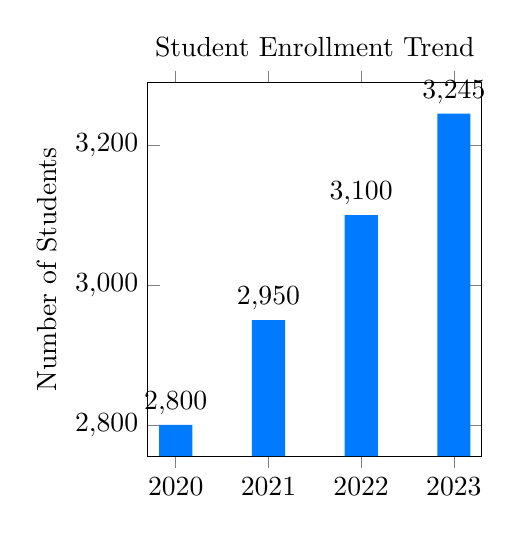
\begin{tikzpicture}
\begin{axis}[
ybar,
width=0.48\textwidth,
height=180pt,
symbolic x coords={2020,2021,2022,2023},
xtick=data,
ylabel={Number of Students},
title={Student Enrollment Trend},
bar width=12pt,
nodes near coords
]
\addplot[fill=chart1, draw=none] coordinates {
(2020,2800)
(2021,2950)
(2022,3100)
(2023,3245)
};
\end{axis}
\end{tikzpicture}
\end{minipage}
\hfill
\begin{minipage}[t]{0.48\textwidth}
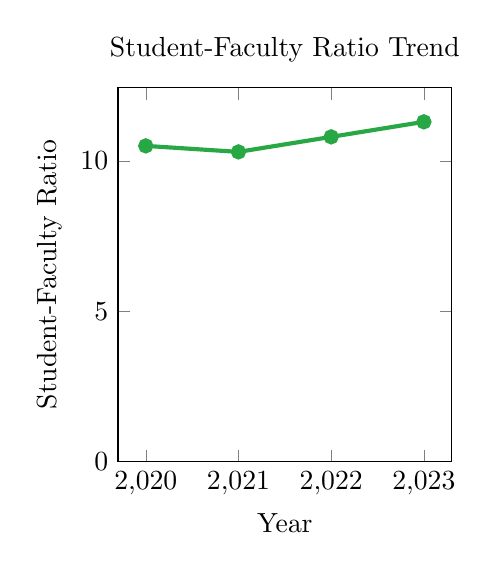
\begin{tikzpicture}
\begin{axis}[
width=0.48\textwidth,
height=180pt,
xlabel={Year},
ylabel={Student-Faculty Ratio},
title={Student-Faculty Ratio Trend},
ymin=0
]
\addplot[color=chart2, mark=*, line width=1.5pt] coordinates {
(2020,10.5)
(2021,10.3)
(2022,10.8)
(2023,11.3)
};
\end{axis}
\end{tikzpicture}
\end{minipage}
\end{center}

\vspace{0.5cm}

\begin{card}
\subsection*{\textcolor{accent}{Department-wise Pass Rates}}
\begin{tabularx}{\textwidth}{@{}lXrr@{}}
\toprule
\textbf{Department} & \textbf{Total Students} & \textbf{Passed} & \textbf{Pass Rate (\%)} \\
\midrule
Computer Science \& Engineering & 650 & 635 & 97.7 \\
Electronics \& Communication Engineering & 580 & 565 & 97.4 \\
Mechanical Engineering & 450 & 420 & 93.3 \\
Civil Engineering & 420 & 395 & 94.0 \\
\bottomrule
\end{tabularx}
\end{card}

\clearpage

% ==============================
% PLACEMENT SECTION
% ==============================
\section{Placement and Career Development}
{\large\textcolor{muted}{Industry Engagement and Student Success}}

\vspace{0.5cm}

\begin{card}
The Placement Cell achieved exceptional results in 2023-24, attracting top-tier companies and securing competitive salary packages for students.
\end{card}

\vspace{0.5cm}

\begin{center}
\begin{minipage}[t]{0.48\textwidth}
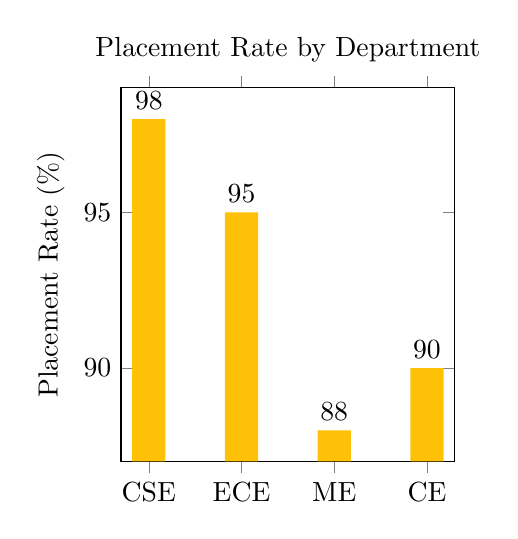
\begin{tikzpicture}
\begin{axis}[
ybar,
width=0.48\textwidth,
height=180pt,
symbolic x coords={CSE,ECE,ME,CE},
xtick=data,
ylabel={Placement Rate (\%)},
title={Placement Rate by Department},
bar width=12pt,
nodes near coords
]
\addplot[fill=chart3, draw=none] coordinates {
(CSE,98)
(ECE,95)
(ME,88)
(CE,90)
};
\end{axis}
\end{tikzpicture}
\end{minipage}
\hfill
\begin{minipage}[t]{0.48\textwidth}
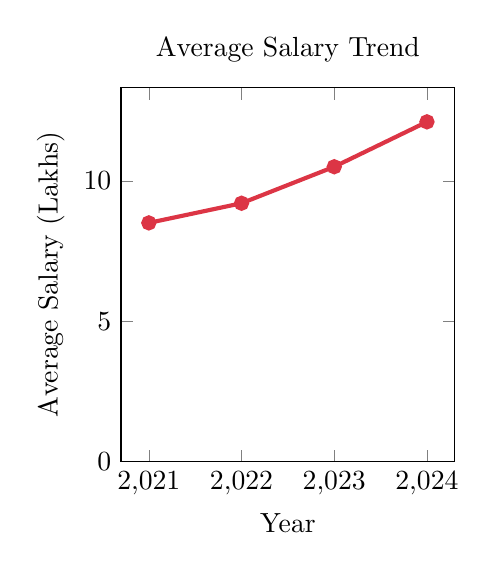
\begin{tikzpicture}
\begin{axis}[
width=0.48\textwidth,
height=180pt,
xlabel={Year},
ylabel={Average Salary (Lakhs)},
title={Average Salary Trend},
ymin=0
]
\addplot[color=chart4, mark=*, line width=1.5pt] coordinates {
(2021,8.5)
(2022,9.2)
(2023,10.5)
(2024,12.1)
};
\end{axis}
\end{tikzpicture}
\end{minipage}
\end{center}

\vspace{0.5cm}

\begin{card}
\subsection*{\textcolor{accent}{Top Recruiting Companies}}
\begin{tabularx}{\textwidth}{@{}lXrr@{}}
\toprule
\textbf{Company} & \textbf{Sector} & \textbf{Offers} & \textbf{Avg Package (Lakhs)} \\
\midrule
TCS & IT Services & 85 & 7.5 \\
Infosys & IT Services & 70 & 7.0 \\
Wipro & IT Services & 60 & 6.8 \\
Reliance Industries & Manufacturing & 25 & 10.0 \\
L\&T & Construction & 20 & 9.5 \\
\bottomrule
\end{tabularx}
\end{card}

\clearpage

% ==============================
% RESEARCH SECTION
% ==============================
\section{Research and Innovation}
{\large\textcolor{muted}{Advancing Knowledge and Impact}}

\vspace{0.5cm}

\begin{card}
Research output increased significantly, with 142 publications and 38 funded projects during 2023-24.
\end{card}

\vspace{0.5cm}

\begin{center}
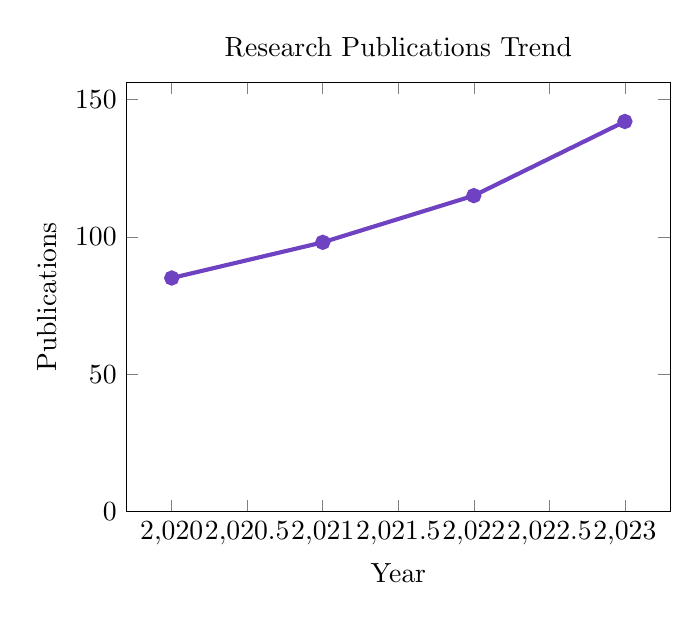
\begin{tikzpicture}
\begin{axis}[
width=0.7\textwidth,
height=200pt,
xlabel={Year},
ylabel={Publications},
title={Research Publications Trend},
ymin=0
]
\addplot[color=chart5, mark=*, line width=1.5pt] coordinates {
(2020,85)
(2021,98)
(2022,115)
(2023,142)
};
\end{axis}
\end{tikzpicture}
\end{center}

\vspace{0.5cm}

\begin{card}
\subsection*{\textcolor{accent}{Funded Projects}}
\begin{tabularx}{\textwidth}{@{}lXrr@{}}
\toprule
\textbf{Project} & \textbf{PI} & \textbf{Agency} & \textbf{Grant (Lakhs)} \\
\midrule
AI for Smart Cities & Dr. A. Sharma & DST & 75.0 \\
Renewable Energy Systems & Dr. B. Singh & MNRE & 60.0 \\
Advanced Materials & Dr. C. Kumar & DRDO & 90.0 \\
Cybersecurity Frameworks & Dr. D. Gupta & MeitY & 50.0 \\
\bottomrule
\end{tabularx}
\end{card}

\clearpage

\end{document}
